Table~\ref{tab:main} gives the main comparison, Fig.~\ref{fig:bars} the steps to first reward, and Table~\ref{tab:tests} the tests we refer to. Steps to first reward is censored at the budget (30k on chains, 100k on rooms), so a value equal to the budget means the reward was never found. All statements are for five seeds and one hyperparameter setting.

\begin{table*}[!t]\centering\caption{Main results (mean $\pm$ std over 5 seeds). Steps to first reward is censored at the step budget (30000 on chains, 100000 on rooms). Bold: lowest mean steps of the column among the six main systems, ties all bold. ``penalty only'' and ``count, no offset'' are the controls for the constant per-step penalty (offset). The two count variants are identical on noise-free tasks by construction. Bottom block: normaliser ablation of Section~\ref{sec:ablations} (standard deviations in \texttt{results/tables/abl\_norm\_long.md}).}\label{tab:main}
\resizebox{\textwidth}{!}{\footnotesize\setlength{\tabcolsep}{3.5pt}\begin{tabular}{lrrrrrrrr}
\hline
System & chain\_10 & chain\_20 & chain\_40 & room\_2 & room\_4 & room\_6 & chain\_20\_tv & room\_4\_tv \\
\hline
\multicolumn{9}{l}{\emph{Steps to first reward}} \\
eps-greedy & 816 $\pm$ 879 & 27752 $\pm$ 5027 & 30000 $\pm$ 0 & 35427 $\pm$ 34281 & 100000 $\pm$ 0 & 100000 $\pm$ 0 & 25007 $\pm$ 11164 & 100000 $\pm$ 0 \\
penalty only & 122 $\pm$ 42 & 618 $\pm$ 119 & 2638 $\pm$ 204 & \textbf{982 $\pm$ 449} & 11921 $\pm$ 723 & 29105 $\pm$ 1775 & 557 $\pm$ 123 & 13231 $\pm$ 371 \\
count, no offset & 5408 $\pm$ 998 & 14402 $\pm$ 1433 & 30000 $\pm$ 0 & 36025 $\pm$ 9848 & 100000 $\pm$ 0 & 100000 $\pm$ 0 & 16227 $\pm$ 3935 & 100000 $\pm$ 0 \\
count (state) & \textbf{88 $\pm$ 60} & \textbf{476 $\pm$ 245} & \textbf{2603 $\pm$ 316} & 1156 $\pm$ 236 & \textbf{11476 $\pm$ 2146} & \textbf{28439 $\pm$ 2256} & \textbf{500 $\pm$ 107} & 11643 $\pm$ 499 \\
count (obs) & \textbf{88 $\pm$ 60} & \textbf{476 $\pm$ 245} & \textbf{2603 $\pm$ 316} & 1156 $\pm$ 236 & \textbf{11476 $\pm$ 2146} & \textbf{28439 $\pm$ 2256} & 612 $\pm$ 142 & \textbf{11142 $\pm$ 2646} \\
RND (guarded) & 525 $\pm$ 351 & 2146 $\pm$ 448 & 5242 $\pm$ 771 & 3905 $\pm$ 576 & 18435 $\pm$ 4082 & 76276 $\pm$ 21269 & 2387 $\pm$ 227 & 15184 $\pm$ 3604 \\
\hline
\multicolumn{9}{l}{\emph{Seeds that found the reward (of 5) / final return}} \\
eps-greedy & 5 / 1.00 $\pm$ 0.00 & 1 / 0.00 $\pm$ 0.00 & 0 / 0.00 $\pm$ 0.00 & 5 / 0.80 $\pm$ 0.45 & 0 / 0.00 $\pm$ 0.00 & 0 / 0.00 $\pm$ 0.00 & 1 / 0.00 $\pm$ 0.00 & 0 / 0.00 $\pm$ 0.00 \\
penalty only & 5 / 1.00 $\pm$ 0.00 & 5 / 1.00 $\pm$ 0.00 & 5 / 1.00 $\pm$ 0.00 & 5 / 1.00 $\pm$ 0.00 & 5 / 1.00 $\pm$ 0.00 & 5 / 1.00 $\pm$ 0.00 & 5 / 1.00 $\pm$ 0.00 & 5 / 1.00 $\pm$ 0.00 \\
count, no offset & 5 / 1.00 $\pm$ 0.00 & 5 / 1.00 $\pm$ 0.00 & 0 / 0.00 $\pm$ 0.00 & 5 / 1.00 $\pm$ 0.00 & 0 / 0.00 $\pm$ 0.00 & 0 / 0.00 $\pm$ 0.00 & 5 / 1.00 $\pm$ 0.00 & 0 / 0.00 $\pm$ 0.00 \\
count (state) & 5 / 1.00 $\pm$ 0.00 & 5 / 1.00 $\pm$ 0.00 & 5 / 1.00 $\pm$ 0.00 & 5 / 1.00 $\pm$ 0.00 & 5 / 1.00 $\pm$ 0.00 & 5 / 1.00 $\pm$ 0.00 & 5 / 1.00 $\pm$ 0.00 & 5 / 1.00 $\pm$ 0.00 \\
count (obs) & 5 / 1.00 $\pm$ 0.00 & 5 / 1.00 $\pm$ 0.00 & 5 / 1.00 $\pm$ 0.00 & 5 / 1.00 $\pm$ 0.00 & 5 / 1.00 $\pm$ 0.00 & 5 / 1.00 $\pm$ 0.00 & 5 / 1.00 $\pm$ 0.00 & 5 / 1.00 $\pm$ 0.00 \\
RND (guarded) & 5 / 1.00 $\pm$ 0.00 & 5 / 1.00 $\pm$ 0.00 & 5 / 1.00 $\pm$ 0.00 & 5 / 0.97 $\pm$ 0.04 & 5 / 1.00 $\pm$ 0.01 & 4 / 0.45 $\pm$ 0.40 & 5 / 1.00 $\pm$ 0.00 & 5 / 1.00 $\pm$ 0.00 \\
\hline
\multicolumn{9}{l}{\emph{RND normaliser variants: mean steps to first reward (seeds that found the reward, of 5)}} \\
RND, clip only & 915 (5) & 2427 (5) & 6493 (5) & 3704 (5) & 17811 (5) & 77950 (4) & 2359 (5) & 19682 (5) \\
RND, warm-up only & 521 (5) & 2051 (5) & 5005 (5) & 3744 (5) & 19474 (5) & 83830 (3) & 2347 (5) & 17106 (5) \\
RND, unguarded (v1) & 6696 (5) & 24510 (1) & 15979 (3) & 42797 (3) & 69777 (2) & 94878 (2) & 13231 (3) & 67356 (2) \\
RND, no normalisation & 64 (5) & 570 (5) & 2620 (5) & 1145 (5) & 13206 (5) & 29808 (5) & 620 (5) & 11439 (5) \\
\hline
\end{tabular}
}\end{table*}

\begin{figure}[!tb]\centering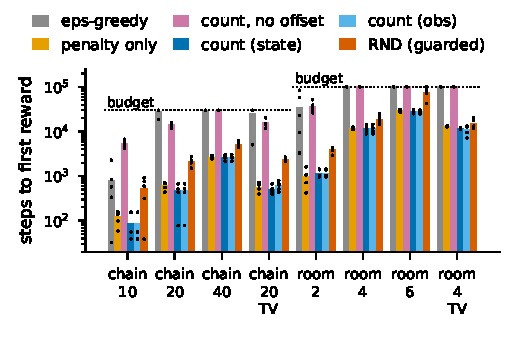
\includegraphics[width=\columnwidth]{generated/bars_main_steps.pdf}\caption{Steps to first reward by system and task, log scale (bars: mean over 5 seeds; dots: the individual seeds; dotted lines: step budget, at which the metric is censored).}\label{fig:bars}\end{figure}

\begin{table}[!tb]\centering\caption{Uncorrected $p$-values on steps to first reward (\texttt{rh compare}, 5 seeds). cnt / RND: paired $t$-test of count (state) against RND (the test registered for H2). pen / RND, cnt / pen, RND / $\epsilon$-gr: Welch tests of penalty only against RND, count (state) against penalty only, and RND against $\epsilon$-greedy.}\label{tab:tests}{\footnotesize\setlength{\tabcolsep}{3.5pt}\begin{tabular}{lrrrr}
\hline
Task & cnt / RND & pen / RND & cnt / pen & RND / $\epsilon$-gr \\
\hline
chain\_10 & \rhval{cmp/main/count-bonus-state/chain_10/steps_to_first_reward/paired_p} & \rhval{cmp/main/step-penalty-only-optimistic-init/chain_10/steps_to_first_reward/welch_p} & \rhval{cmp/offset_control/count-bonus-state/chain_10/steps_to_first_reward/welch_p} & \rhval{cmp/main/epsilon-greedy-q-learning/chain_10/steps_to_first_reward/welch_p} \\
chain\_20 & \rhval{cmp/main/count-bonus-state/chain_20/steps_to_first_reward/paired_p} & \rhval{cmp/main/step-penalty-only-optimistic-init/chain_20/steps_to_first_reward/welch_p} & \rhval{cmp/offset_control/count-bonus-state/chain_20/steps_to_first_reward/welch_p} & \rhval{cmp/main/epsilon-greedy-q-learning/chain_20/steps_to_first_reward/welch_p} \\
chain\_40 & \rhval{cmp/main/count-bonus-state/chain_40/steps_to_first_reward/paired_p} & \rhval{cmp/main/step-penalty-only-optimistic-init/chain_40/steps_to_first_reward/welch_p} & \rhval{cmp/offset_control/count-bonus-state/chain_40/steps_to_first_reward/welch_p} & \rhval{cmp/main/epsilon-greedy-q-learning/chain_40/steps_to_first_reward/welch_p} \\
room\_2 & \rhval{cmp/main/count-bonus-state/room_2/steps_to_first_reward/paired_p} & \rhval{cmp/main/step-penalty-only-optimistic-init/room_2/steps_to_first_reward/welch_p} & \rhval{cmp/offset_control/count-bonus-state/room_2/steps_to_first_reward/welch_p} & \rhval{cmp/main/epsilon-greedy-q-learning/room_2/steps_to_first_reward/welch_p} \\
room\_4 & \rhval{cmp/main/count-bonus-state/room_4/steps_to_first_reward/paired_p} & \rhval{cmp/main/step-penalty-only-optimistic-init/room_4/steps_to_first_reward/welch_p} & \rhval{cmp/offset_control/count-bonus-state/room_4/steps_to_first_reward/welch_p} & \rhval{cmp/main/epsilon-greedy-q-learning/room_4/steps_to_first_reward/welch_p} \\
room\_6 & \rhval{cmp/main/count-bonus-state/room_6/steps_to_first_reward/paired_p} & \rhval{cmp/main/step-penalty-only-optimistic-init/room_6/steps_to_first_reward/welch_p} & \rhval{cmp/offset_control/count-bonus-state/room_6/steps_to_first_reward/welch_p} & \rhval{cmp/main/epsilon-greedy-q-learning/room_6/steps_to_first_reward/welch_p} \\
chain\_20\_tv & \rhval{cmp/main/count-bonus-state/chain_20_tv/steps_to_first_reward/paired_p} & \rhval{cmp/main/step-penalty-only-optimistic-init/chain_20_tv/steps_to_first_reward/welch_p} & \rhval{cmp/offset_control/count-bonus-state/chain_20_tv/steps_to_first_reward/welch_p} & \rhval{cmp/main/epsilon-greedy-q-learning/chain_20_tv/steps_to_first_reward/welch_p} \\
room\_4\_tv & \rhval{cmp/main/count-bonus-state/room_4_tv/steps_to_first_reward/paired_p} & \rhval{cmp/main/step-penalty-only-optimistic-init/room_4_tv/steps_to_first_reward/welch_p} & \rhval{cmp/offset_control/count-bonus-state/room_4_tv/steps_to_first_reward/welch_p} & \rhval{cmp/main/epsilon-greedy-q-learning/room_4_tv/steps_to_first_reward/welch_p} \\
\hline
\end{tabular}
}\end{table}

\textbf{H1 (both bonuses beat $\epsilon$-greedy on the larger tasks): supported as stated, but the controls show that neither bonus is the cause.} The count bonus found the reward in all five seeds on every task. $\epsilon$-greedy found it in no seed on chain\_40, room\_4 and room\_6 and in one of five on chain\_20: with all Q-values at zero it is a uniform random walk until the first reward. The RND bonus found the reward in every seed except one on room\_6; its mean is 5242 steps on chain\_40 and 76276 on room\_6, where $\epsilon$-greedy sits at the budget (Welch $p<0.001$ and $p=0.067$, Table~\ref{tab:tests}). On chain\_10 and room\_2, where $\epsilon$-greedy does find the reward, RND does not differ from it at the 0.05 level ($p=0.521$ and $0.109$). The controls change the reading. ``Penalty only'' has the same constant per-step penalty as the bonus systems and no bonus: it finds the reward in all seeds on every task, and its means are close to the count bonus on chain\_40, room\_4 and room\_6 (2638 against 2603, 11921 against 11476, 29105 against 28439). On all six noise-free tasks the gap between the two is below the larger of their standard deviations and Welch $p\geq0.288$. The count bonus without the offset finds the reward in no seed on chain\_40, room\_4 and room\_6. Hence the gain over $\epsilon$-greedy is explained by the optimistic offset, which the $\epsilon$-greedy baseline does not have; the data give no evidence that counts add speed beyond it on the noise-free tasks. The one exception is room\_4\_tv, where the state count is faster than the penalty-only control (11643 against 13231 steps, $p<0.001$ uncorrected). We read it with caution: the penalty-only control cannot see the token, yet its own time differs between room\_4 and room\_4\_tv ($p=0.011$, Table~\ref{tab:tv}).

\textbf{H2 (counts at least as fast as RND, noise-free): supported, but it is not evidence for the count signal.} The count bonus is faster than RND on all six noise-free tasks, with paired $p<0.05$ on each (Table~\ref{tab:tests}); four of the six would survive a Bonferroni correction over the six tasks. However, the penalty-only control is faster than RND by similar margins (2146 against 618 steps on chain\_20, 18435 against 11921 on room\_4, 76276 against 29105 on room\_6; Welch $p<0.05$ on five of the six noise-free tasks, $p=0.062$ on chain\_10). So H2 holds because the RND-style signal costs time relative to no bonus, not because the count signal gains any.

\textbf{Where RND fails.} Room\_6 is the worst case: one seed never finds the reward, the spread is large ($76276\pm21269$ steps), and because the reward is found late the final return is only $0.45\pm0.40$. Along the chains the absolute gap to the penalty-only control grows (525 against 122, 2146 against 618, 5242 against 2638) while the relative gap shrinks; the rooms show no monotone pattern.

\begin{table}[!tb]\centering\caption{TV tasks: share of steps on the TV cell (mean $\pm$ std), mean steps to first reward on the noise-free twin (``twin'') and on the TV task (``TV''), and Welch $p$ between the two (5 seeds).}\label{tab:tv}{\footnotesize\setlength{\tabcolsep}{4pt}\begin{tabular}{lrrr}
\hline
System & TV share & twin & TV \\
\hline
\multicolumn{4}{l}{\emph{chain\_20\_tv (twin: chain\_20)}} \\
eps-greedy & 0.214 $\pm$ 0.003 & 27752 & 25007 \\
penalty only & 0.054 $\pm$ 0.001 & 618 & 557 \\
count (state) & 0.054 $\pm$ 0.001 & 476 & 500 \\
count (obs) & 0.055 $\pm$ 0.001 & 476 & 612 \\
RND (guarded) & 0.062 $\pm$ 0.003 & 2146 & 2387 \\
\hline
\multicolumn{4}{l}{\emph{room\_4\_tv (twin: room\_4)}} \\
eps-greedy & 0.035 $\pm$ 0.001 & 100000 & 100000 \\
penalty only & 0.021 $\pm$ 0.010 & 11921 & 13231 \\
count (state) & 0.013 $\pm$ 0.001 & 11476 & 11643 \\
count (obs) & 0.023 $\pm$ 0.001 & 11476 & 11142 \\
RND (guarded) & 0.025 $\pm$ 0.001 & 18435 & 15184 \\
\hline
\end{tabular}
}\end{table}

\textbf{H3 (noisy TV delays RND, not the state count): not supported.} RND's time to first reward is 2387 steps on chain\_20\_tv against 2146 on chain\_20 ($p=0.324$) and 15184 on room\_4\_tv against 18435 on room\_4 ($p=0.219$): above the twin in the mean on one task, below on the other, neither beyond the seed spread (Table~\ref{tab:tv}). The observation count is not delayed either ($p=0.323$ and $0.832$). For RND this is the expected outcome, not a surprise: its target is a deterministic function of the observation and our token set is finite, so both the RND error and the observation count on the TV decay with visits \cite{burda2018exploration}. The systems that see the token do spend slightly more time on the TV than the state count on room\_4\_tv ($0.025\pm0.001$ for RND and $0.023\pm0.001$ for the observation count against $0.013\pm0.001$), and the $K$ sweep in Section~\ref{sec:ablations} confirms that this share depends on the token. The large TV share of $\epsilon$-greedy on chain\_20\_tv (0.214) is unrelated to novelty: the TV cell is next to the start, where a random walk stays.

\textbf{What the numbers do not show.} They do not show that count or RND bonuses are useless in general: the tasks are deterministic and small, so optimism alone explores systematically. Nor can they show a noisy-TV failure: forward-model curiosity is not among our systems.
